\documentclass[a4paper,12pt]{article}
%%% Работа с русским языком % для pdfLatex
\usepackage{cmap}					% поиск в~PDF
\usepackage{mathtext} 				% русские буквы в~фомулах
\usepackage[T2A]{fontenc}			% кодировка
\usepackage[utf8]{inputenc}			% кодировка исходного текста
\usepackage[english,russian]{babel}	% локализация и переносы
\usepackage{indentfirst} 			% отступ 1 абзаца

%%% Работа с русским языком % для XeLatex
%\usepackage[english,russian]{babel}   %% загружает пакет многоязыковой вёрстки
%\usepackage{fontspec}      %% подготавливает загрузку шрифтов Open Type, True Type и др.
%\defaultfontfeatures{Ligatures={TeX},Renderer=Basic}  %% свойства шрифтов по умолчанию
%\setmainfont[Ligatures={TeX,Historic}]{Times New Roman} %% задаёт основной шрифт документа
%\setsansfont{Comic Sans MS}                    %% задаёт шрифт без засечек
%\setmonofont{Courier New}
%\usepackage{indentfirst}
%\frenchspacing

%%% Дополнительная работа с математикой
\usepackage{amsfonts,amssymb,amsthm,mathtools}
\usepackage{amsmath}
\usepackage{icomma} % "Умная" запятая: $0,2$ --- число, $0, 2$ --- перечисление
\usepackage{upgreek}

%% Номера формул
%\mathtoolsset{showonlyrefs=true} % Показывать номера только у тех формул, на которые есть \eqref{} в~тексте.

%%% Страница
\usepackage{extsizes} % Возможность сделать 14-й шрифт

%% Шрифты
\usepackage{euscript}	 % Шрифт Евклид
\usepackage{mathrsfs} % Красивый матшрифт

%% Свои команды
\DeclareMathOperator{\sgn}{\mathop{sgn}} % создание новой конанды \sgn (типо как \sin)
\usepackage{csquotes} % ещё одна штука для цитат
\newcommand{\pd}[2]{\ensuremath{\cfrac{\partial #1}{\partial #2}}} % частная производная
\newcommand{\abs}[1]{\ensuremath{\left|#1\right|}} % модуль
\renewcommand{\phi}{\ensuremath{\varphi}} % греческая фи
\newcommand{\pogk}[1]{\!\left(\cfrac{\sigma_{#1}}{#1}\right)^{\!\!\!2}\!} % для погрешностей

% Ссылки
\usepackage{color} % подключить пакет color
% выбрать цвета
\definecolor{BlueGreen}{RGB}{49,152,255}
\definecolor{Violet}{RGB}{120,80,120}
% назначить цвета при подключении hyperref
\usepackage[unicode, colorlinks, urlcolor=blue, linkcolor=blue, pagecolor=blue, citecolor=blue]{hyperref} %синие ссылки
%\usepackage[unicode, colorlinks, urlcolor=black, linkcolor=black, pagecolor=black, citecolor=black]{hyperref} % для печати (отключить верхний!)


%% Перенос знаков в~формулах (по Львовскому)
\newcommand*{\hm}[1]{#1\nobreak\discretionary{}
	{\hbox{$\mathsurround=0pt #1$}}{}}

%%% Работа с картинками
\usepackage{graphicx}  % Для вставки рисунков
\graphicspath{{images/}{images2/}}  % папки с картинками
\setlength\fboxsep{3pt} % Отступ рамки \fbox{} от рисунка
\setlength\fboxrule{1pt} % Толщина линий рамки \fbox{}
\usepackage{wrapfig} % Обтекание рисунков и таблиц текстом
\usepackage{multicol}

%%% Работа с таблицами
\usepackage{array,tabularx,tabulary,booktabs} % Дополнительная работа с таблицами
\usepackage{longtable}  % Длинные таблицы
\usepackage{multirow} % Слияние строк в~таблице
\usepackage{caption}
\captionsetup{labelsep=period, labelfont=bf}

%%% Оформление
\usepackage{indentfirst} % Красная строка
%\setlength{\parskip}{0.3cm} % отступы между абзацами
%%% Название разделов
\usepackage{titlesec}
\titlelabel{\thetitle.\quad}
\renewcommand{\figurename}{\textbf{Рис.}}		%Чтобы вместо figure под рисунками писал "рис"
\renewcommand{\tablename}{\textbf{Таблица}}		%Чтобы вместо table над таблицами писал Таблица

%%% Теоремы
\theoremstyle{plain} % Это стиль по умолчанию, его можно не переопределять.
\newtheorem{theorem}{Теорема}[section]
\newtheorem{proposition}[theorem]{Утверждение}

\theoremstyle{definition} % "Определение"
\newtheorem{definition}{Определение}[section]
\newtheorem{corollary}{Следствие}[theorem]
\newtheorem{problem}{Задача}[section]

\theoremstyle{remark} % "Примечание"
\newtheorem*{nonum}{Решение}
\newtheorem{zamech}{Замечание}[theorem]

%%% Правильные мат. символы для русского языка
\renewcommand{\epsilon}{\ensuremath{\varepsilon}}
\renewcommand{\phi}{\ensuremath{\varphi}}
\renewcommand{\kappa}{\ensuremath{\varkappa}}
\renewcommand{\le}{\ensuremath{\leqslant}}
\renewcommand{\leq}{\ensuremath{\leqslant}}
\renewcommand{\ge}{\ensuremath{\geqslant}}
\renewcommand{\geq}{\ensuremath{\geqslant}}
\renewcommand{\emptyset}{\varnothing}

\usepackage{bm} %жирный греческий шрифт
%\usepackage{ulem}

\graphicspath{{images}}

\renewcommand{\baselinestretch}{1.3}

\title{vopr}
\author{Георгий Демьянов}
\date{today}
\usepackage[left=1.27cm,right=1.27cm,top=1.27cm,bottom=2cm]{geometry}

\begin{document}

\begin{titlepage}
\begin{center} 
 
\large Московский физико-технический институт\\
Факультет молекулярной и химической физики\\
\vspace{7cm}
\huge \textbf{Построение кривой титрования CH$_3$COOH сильным основанием NaOH}\\
\end{center} 

\vspace{7.5cm}
{\par \raggedleft \large \emph{Выполнил:}\\ студент 2 курса\\ 642 группы ФМХФ\\ Демьянов Георгий\\ Сергеевич \par}
\begin{center}
\vfill Москва 2017
\end{center}
\end{titlepage}
\newpage
\setcounter{page}{2}

\textit{Задание:} титруем 8 мл 0.05 н. CH$_3$COOH 0.05 н. NaOH. K$_{\text{д}} = 1.86\cdot 10^{-5}$. Построить кривую титрования, подобрать индикатор для данного процесса. Привести расчеты всех точек титрования.

В качестве индикатора можно выбрать метиловый оранжевый.
\begin{enumerate}
	\item V(NaOH)$_{\text{доб}}$ = 0 мл
	\begin{center}
	$\overset{C - x}{\text{CH$_3$COOH}}$ $\leftrightarrows$ $\overset{x}{\text{CH}_3\text{COO}^-}$ + $\overset{x}{\text{H}^+}$
	\end{center}
	$K_{\text{д}} = \cfrac{x^2}{C-x}$ $\Rightarrow$ $x = 9.55\cdot 10^{-4}$ моль/л $\Rightarrow$ pH $= 3.02$
	\item Далее до добавления 8 мл NaOH раствор является буферным. Формула для расчета pH буферного раствора:
	\begin{equation}\label{phb}
	pH = pK + \lg{\cfrac{C_{\text{соли}}}{C_{\text{к-ты}}}}
	\end{equation}
	Запишем концентрацию кислоты при добавлении $V$ л NaOH:
	$$C(CH_3COOH) = \frac{0.05(0.008-V)}{0.008+V}$$
	Тогда концентрация соли в растворе
	$$C(CH_3COONa) = \cfrac{0.05V}{0.008+V}$$
	Подставляя данные уравнения в формулу \eqref{phb}, получим\\
	$
	pH=pK+\lg\cfrac{0.05V}{0.05(0.008-V)}
	$\\
	Отсюда
	\begin{equation}
	pH=pK-\lg\left(\cfrac{8}{V(NaOH)_{\text{доб}}}-1 \right)
	\end{equation}
	Т.к. формула \eqref{phb} была выведена в приближении, что концентрации соли и кислоты велики, то при очень малых порциях $V(NaOH)_{\text{доб}}$ (до $V(NaOH)_{\text{доб}}$ = 0.4 мл) будем считать зависимость линейной.
	\item $V(NaOH)_{\text{доб}}$ = 8 мл. В колбе находится только соль $CH_3COONa$.\\
	Запишем уравнение гидролиза
	$$
	CH_3COO^- + H_2O\leftrightarrows CH_3COOH + OH^-
	$$
	$K_{\text{г}} = \frac{K_w}{K_{\text{д}}} = 5.38 \cdot 10^{-10}.$ Отсюда аналогично подсчетам в п.1, получаем\\
	$
	[OH^-] = 3.67\cdot 10^{-6} \text{ моль/л}
	$, откуда
	$$
	pH=14+\lg[OH^-]=8.56
	$$
	\item При дальнейшем добавлении NaOH можно считать вклад гидролиза равным нулю (вследствие смещения равновесия). Тогда концентрацию $OH^-$ ионов можно найти из концентрации добавленного после точки эквивалента NaOH: $[OH^-] = \cfrac{0.05\left(V(NaOH)_{\text{доб}}-8\right)}{V(NaOH)_{\text{доб}}+8}$. Отсюда
	\begin{equation}
	pH=14+\lg\cfrac{0.05\left(V(NaOH)_{\text{доб}}-8\right)}{V(NaOH)_{\text{доб}}+8}
	\end{equation}
\end{enumerate}
Окончательно нанесем все функции и точки на плоскость и построим график:
\begin{comment}
\begin{figure}
	\centering
	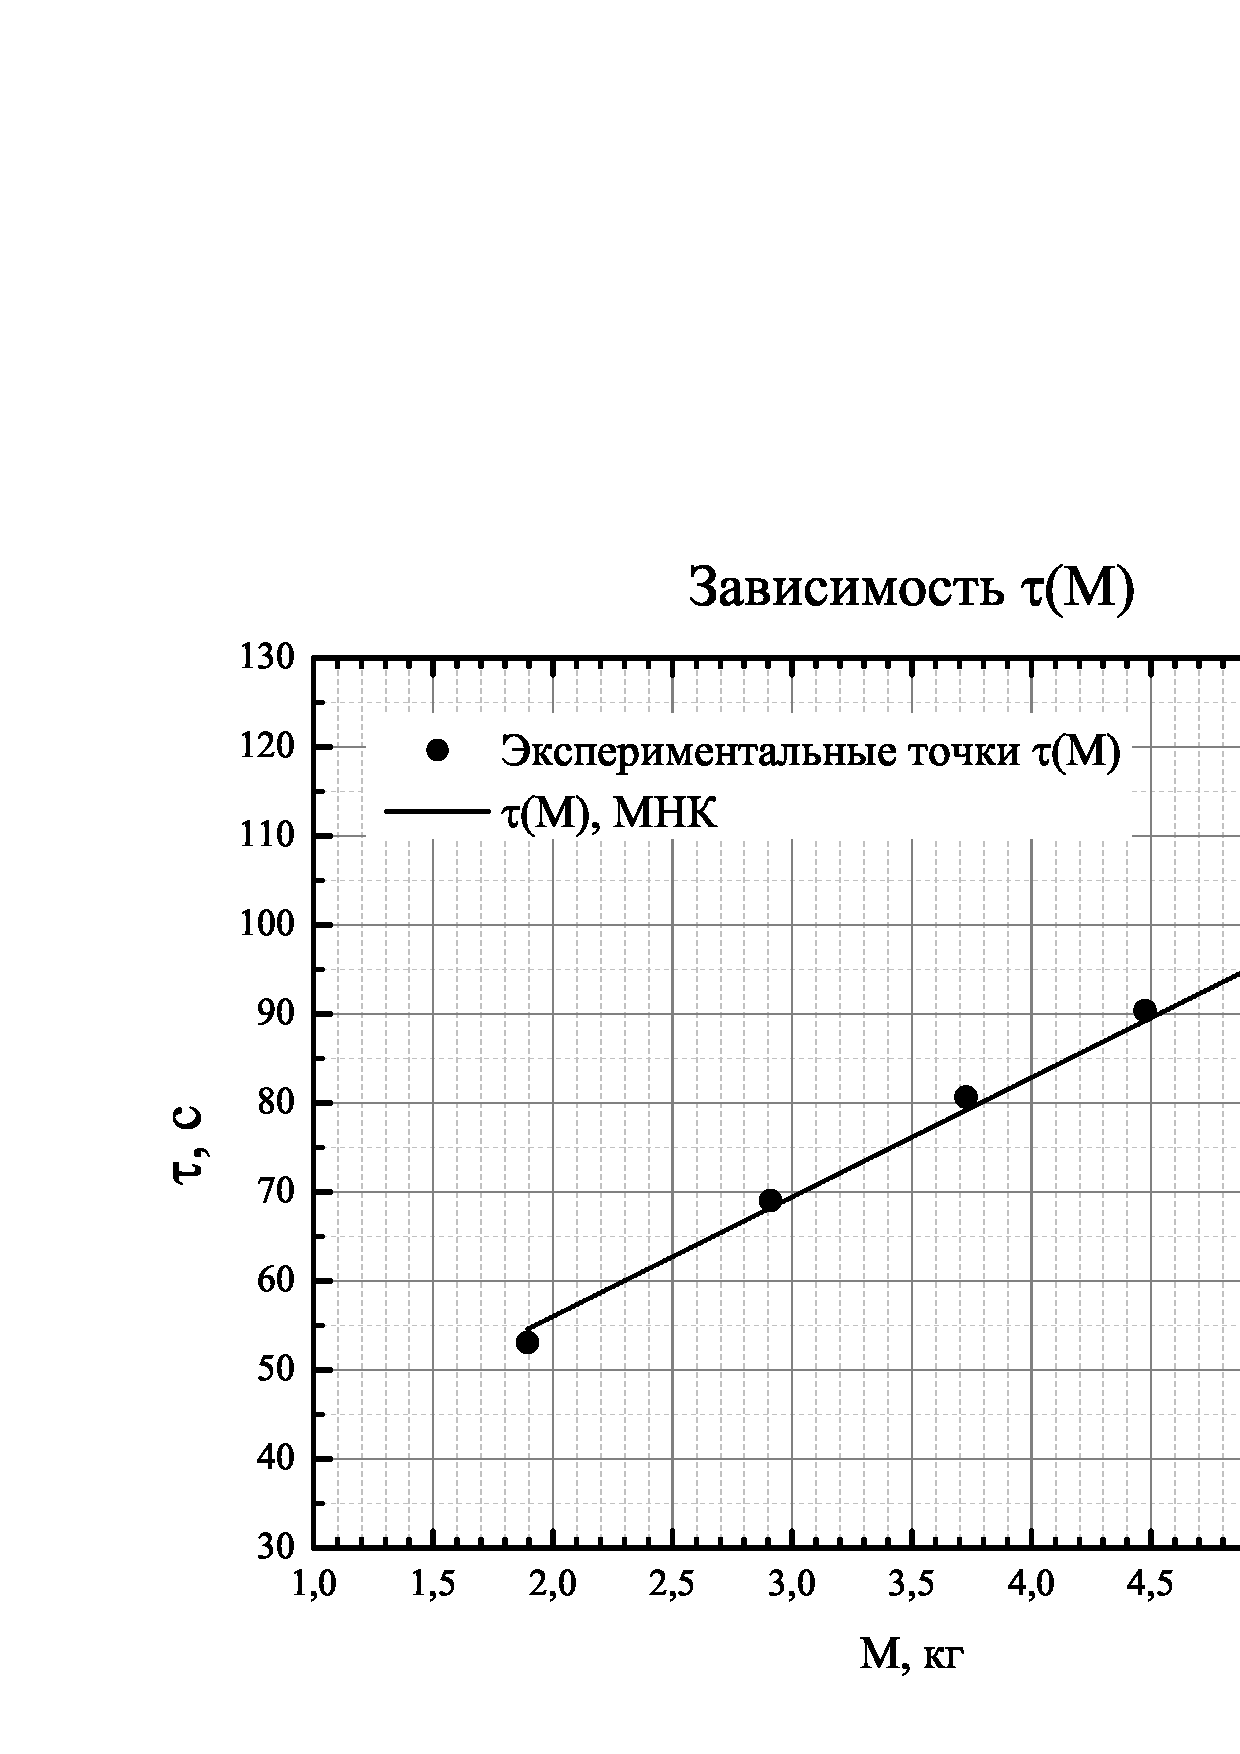
\includegraphics[angle=90, width=\linewidth]{graph}
	\caption{Зависимость $pH (V(NaOH)_{\text{доб}})$}
	\label{Fig:graph}
\end{figure}
\end{comment}
\begin{sidewaysfigure}
	
	\centerline{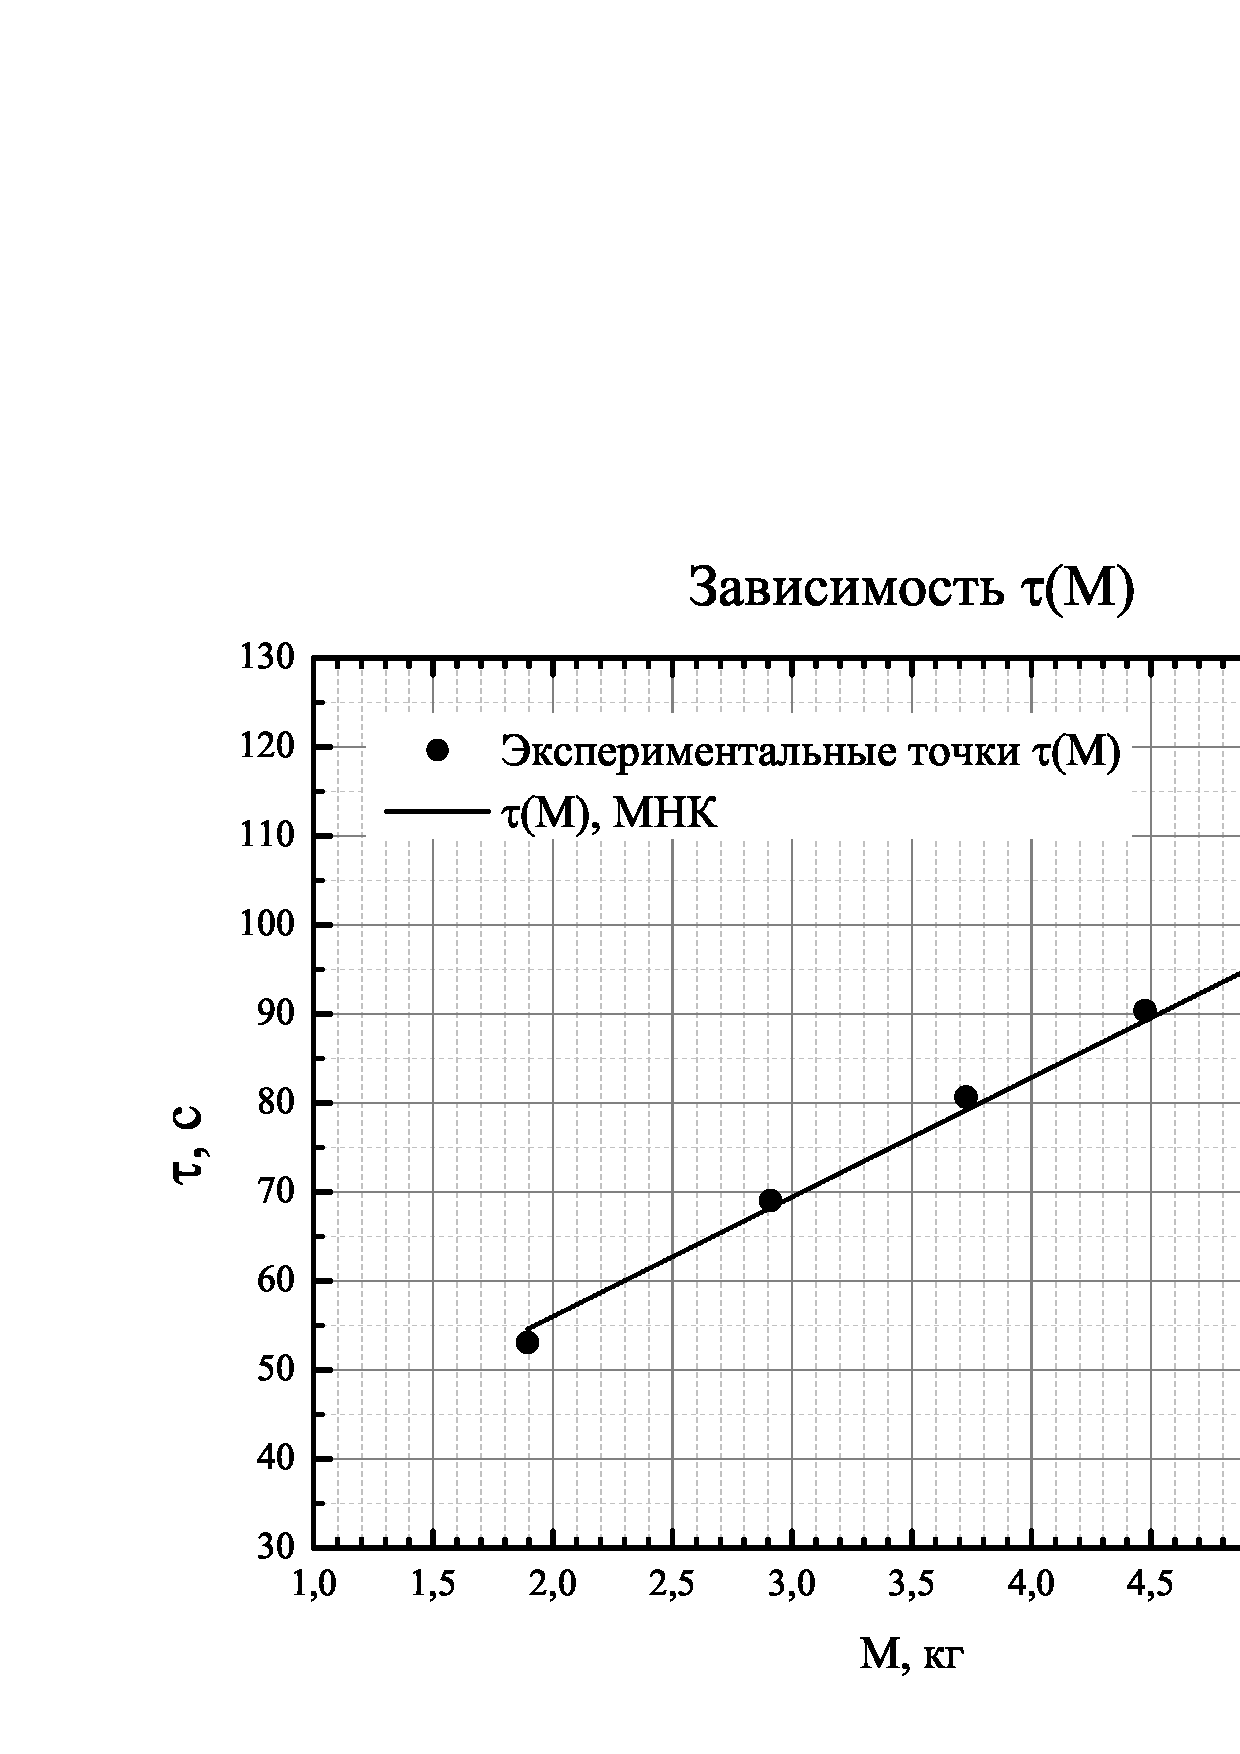
\epsfig{file=graph.pdf, scale=0.75}}
	
	\caption{Зависимость $pH (V(NaOH)_{\text{доб}})$}
	
	\label{label_this_fig}
	
\end{sidewaysfigure}















\end{document}